\documentclass[mathserif]{beamer}
\usepackage[utf8]{inputenc}
\usepackage{amsmath}
\usepackage{amsfonts}
\usepackage{amssymb}
\usepackage{arydshln}
\usepackage{graphicx}
\usepackage{float}
\usepackage{picture}
\usepackage{dcolumn}
\usepackage{textpos}
\usepackage{graphicx}
\usepackage{subcaption}
\usepackage{tikz}
\usepackage{pgfplots}

\setbeamercolor{structure}{fg=grey}
\usetheme[sectionpage=progressbar, progressbar=frametitle]{metropolis}

\definecolor{prettyBlue}{HTML}{2196F3}
\setbeamercolor{progress bar}{fg=prettyBlue, bg=gray}

%Information to be included in the title page:
\title{Development of a Pendulum Control System}
\author{Thomas S. Christensen \\ Mikkel S. Jaedicke\\}

\institute{University of Southern Denmark}
\date{Jan, 2018} 

\addtobeamertemplate{frametitle}{}{%
\begin{textblock*}{200mm}(\textwidth-1.5cm,-0.8cm)

\includegraphics[scale=0.15]{graphics/sdu_logo}
\end{textblock*}}

\begin{document}

\begin{frame}[t]\frametitle{~}
\maketitle
\end{frame}

\begin{frame}[c]\frametitle{Agenda}
\setbeamertemplate{section in toc}[sections numbered]
\tableofcontents[hideallsubsections]
\end{frame}


\section{Introduction}

\begin{frame}[c]\frametitle{System Overview}

\centering
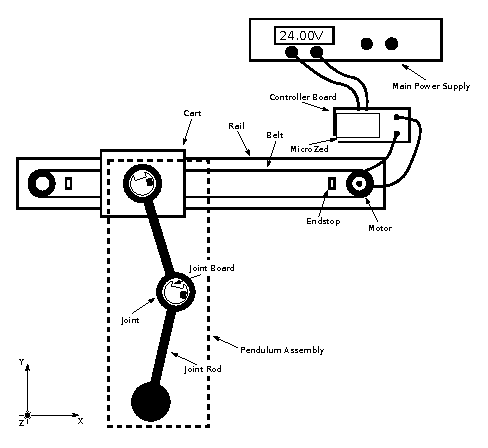
\includegraphics[scale=1]{graphics/system_overview}
\end{frame}

\begin{frame}[c]\frametitle{Implemented System}
\centering
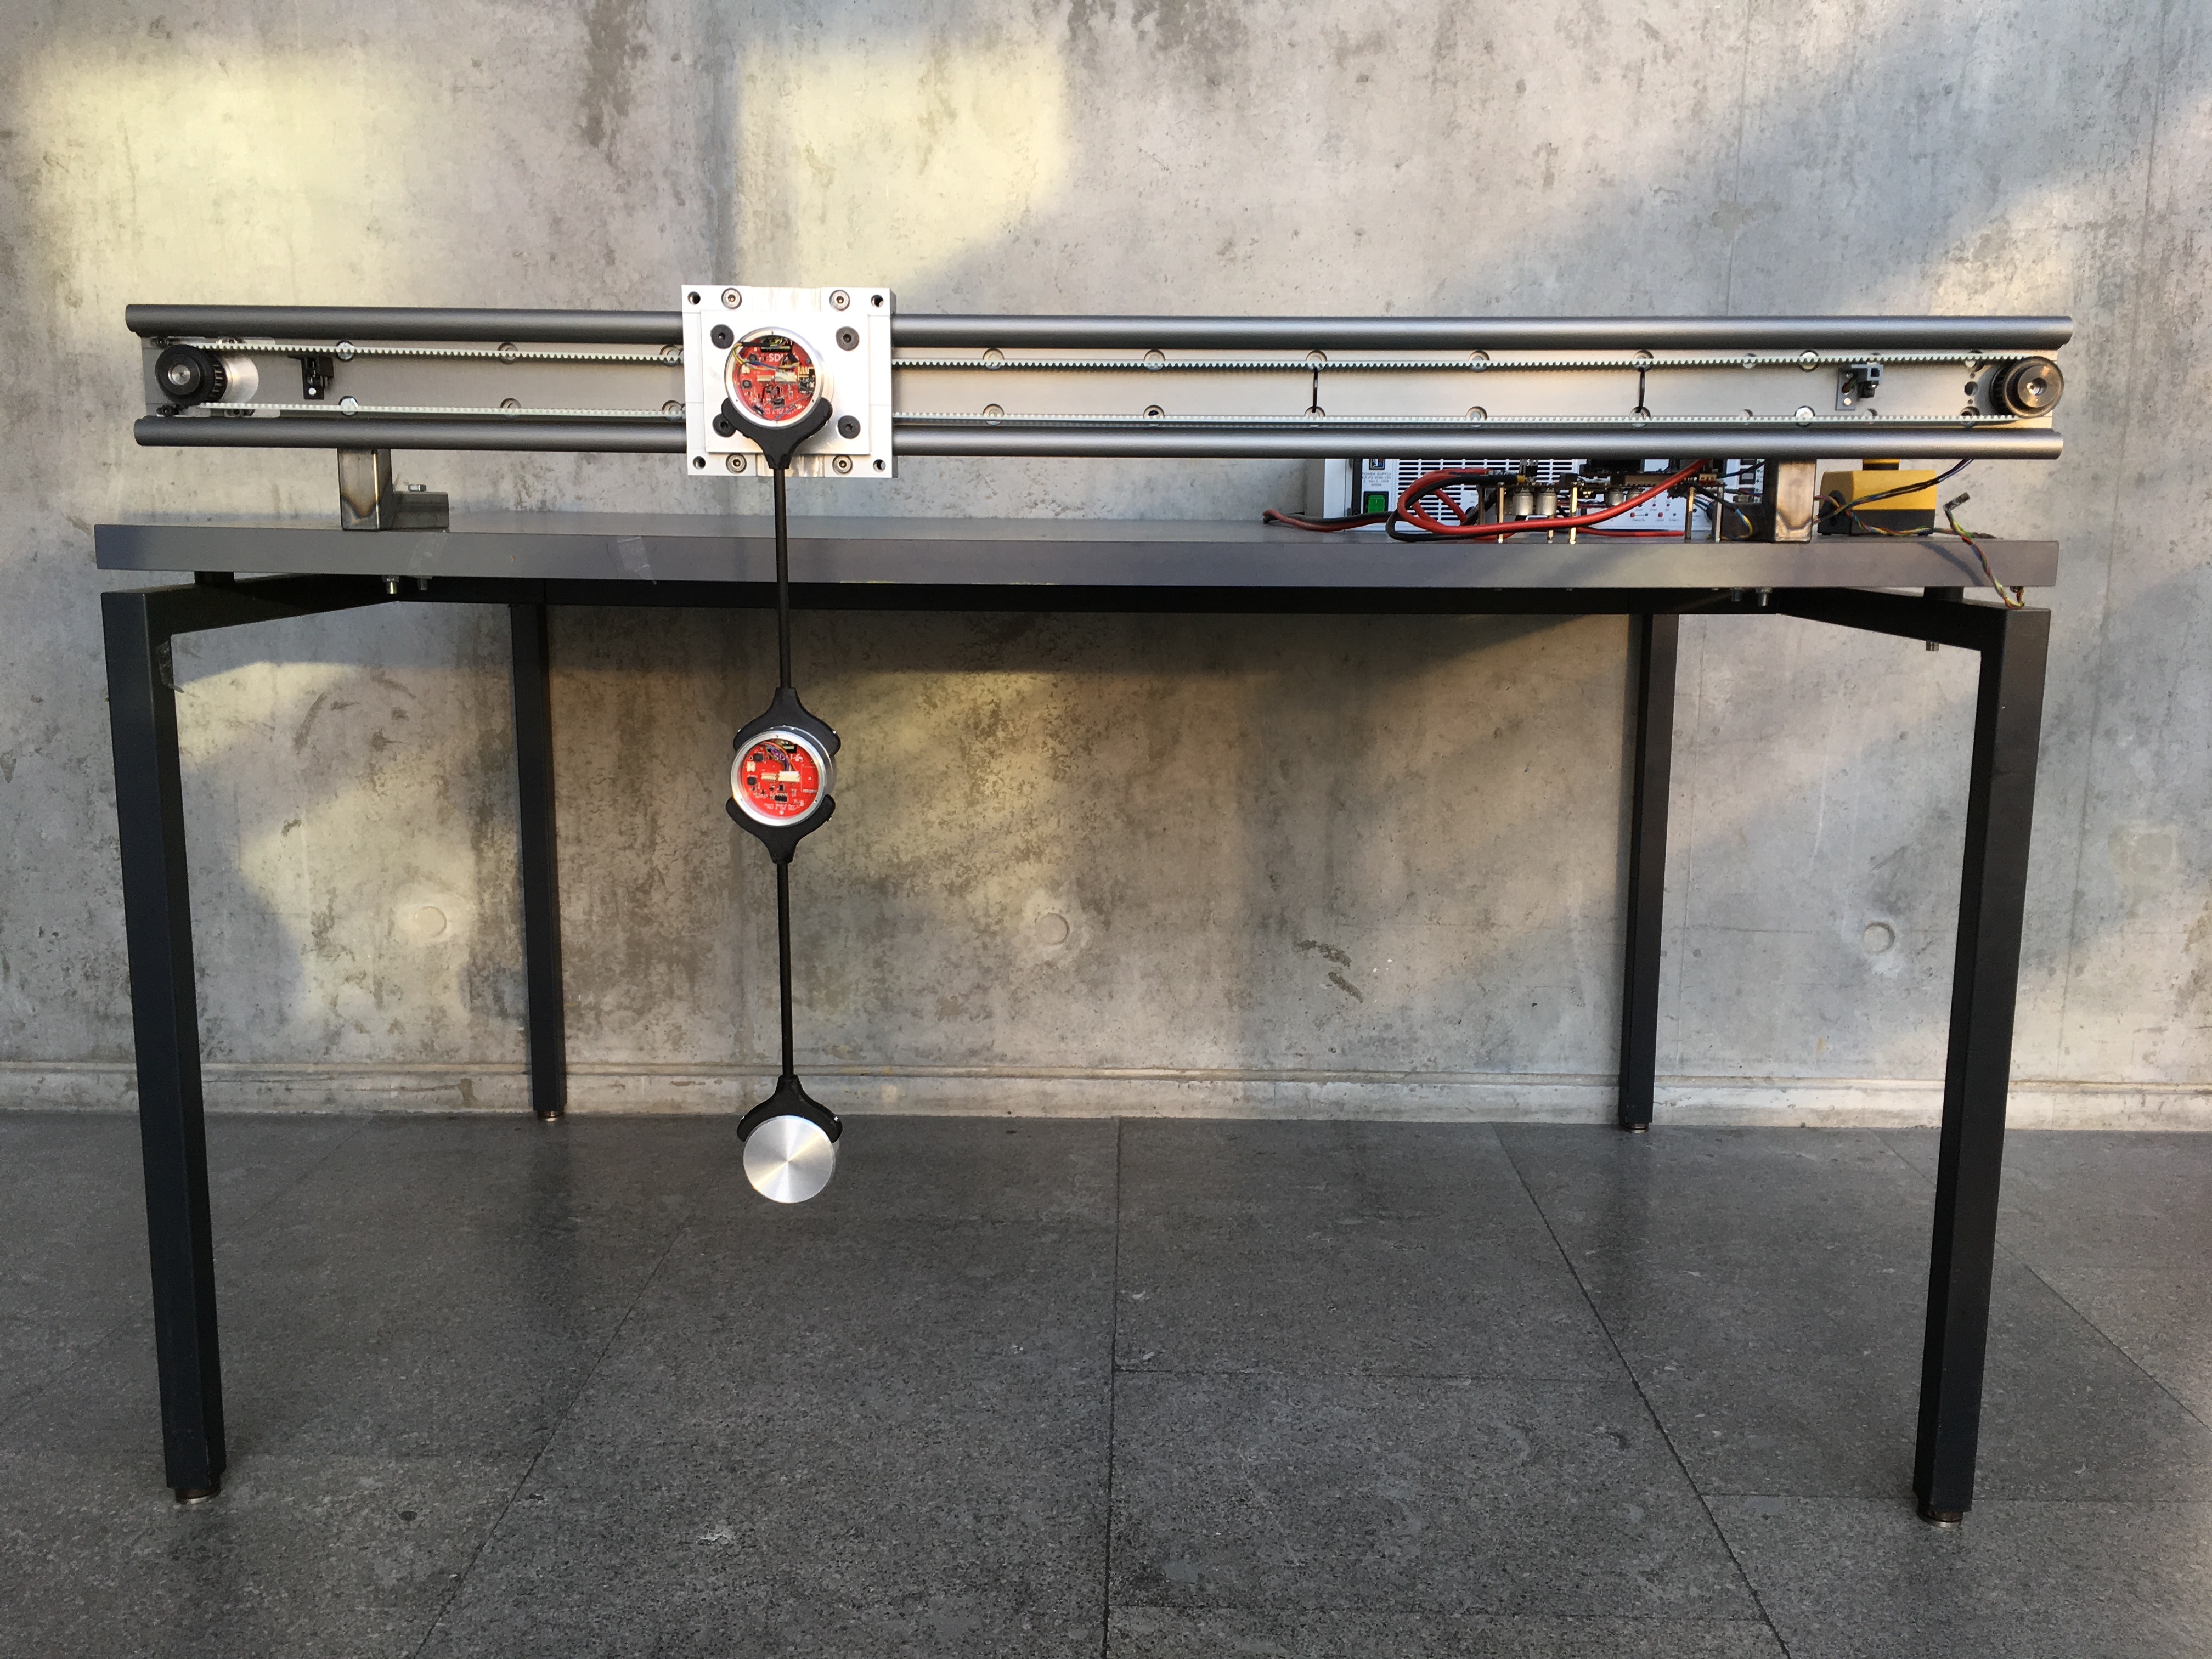
\includegraphics[width=0.9\textwidth]{graphics/full_system_finish}
\end{frame}

\begin{frame}[c]\frametitle{Workflow}
\centering
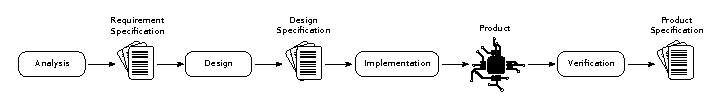
\includegraphics[width=\textwidth]{graphics/workflow}    
\end{frame}


\section{Analysis}

\begin{frame}[t]\frametitle{Analysis}
    Something here?!
\end{frame}

\begin{frame}[c]\frametitle{Requirement Specification}

\textbf{Functional:}
\begin{enumerate}
	\item System should consists of a double pendulum mounted on a moveable cart.
	\item Cart should be actuated by the Maxon 148867. 
	\item The pendulum system should be controlled by a MicroZed.
	\item \alert{Position of the cart and joint angles should be measured.}
\end{enumerate}

\end{frame}

\section{Design}

\begin{frame}{Mechanical Design}
	\begin{figure}
	\centering
	\begin{subfigure}{.5\textwidth}
	  \centering
	  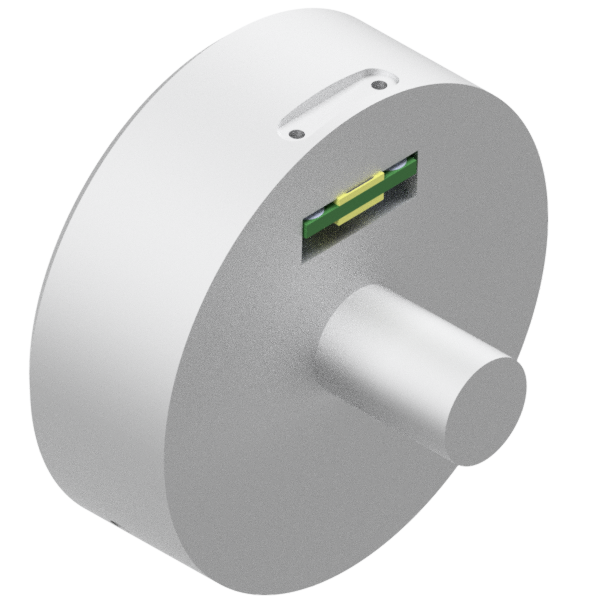
\includegraphics[width=.9\linewidth]{graphics/joint_read_side}
	\end{subfigure}%
	\begin{subfigure}{.5\textwidth}
	  \centering
	  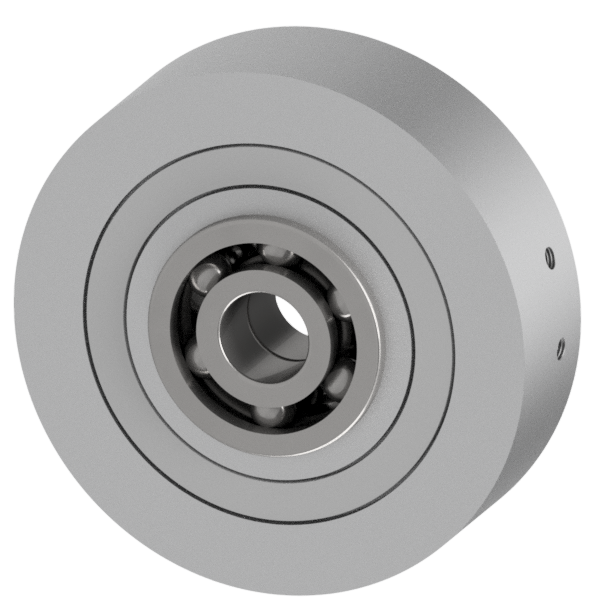
\includegraphics[width=.9\linewidth]{graphics/joint_mag_assembly}
	\end{subfigure}
	\end{figure}
\end{frame}

\begin{frame}[c]\frametitle{Electrical Design}
	\begin{itemize}
    	\item Encoder
    	\item Wireless Communication
    	\item Microcontroller
    	\item Power Delivery
    \end{itemize}    
\end{frame}

\begin{frame}[c]\frametitle{Electrical Design}
	\begin{itemize}
    	\item Encoder
    	\item Wireless Communication
    	\item Microcontroller
    	\item \alert{Power Delivery}
    \end{itemize}    
\end{frame}

\begin{frame}[c]\frametitle{Power Delivery}
	\centering
	\vfill
    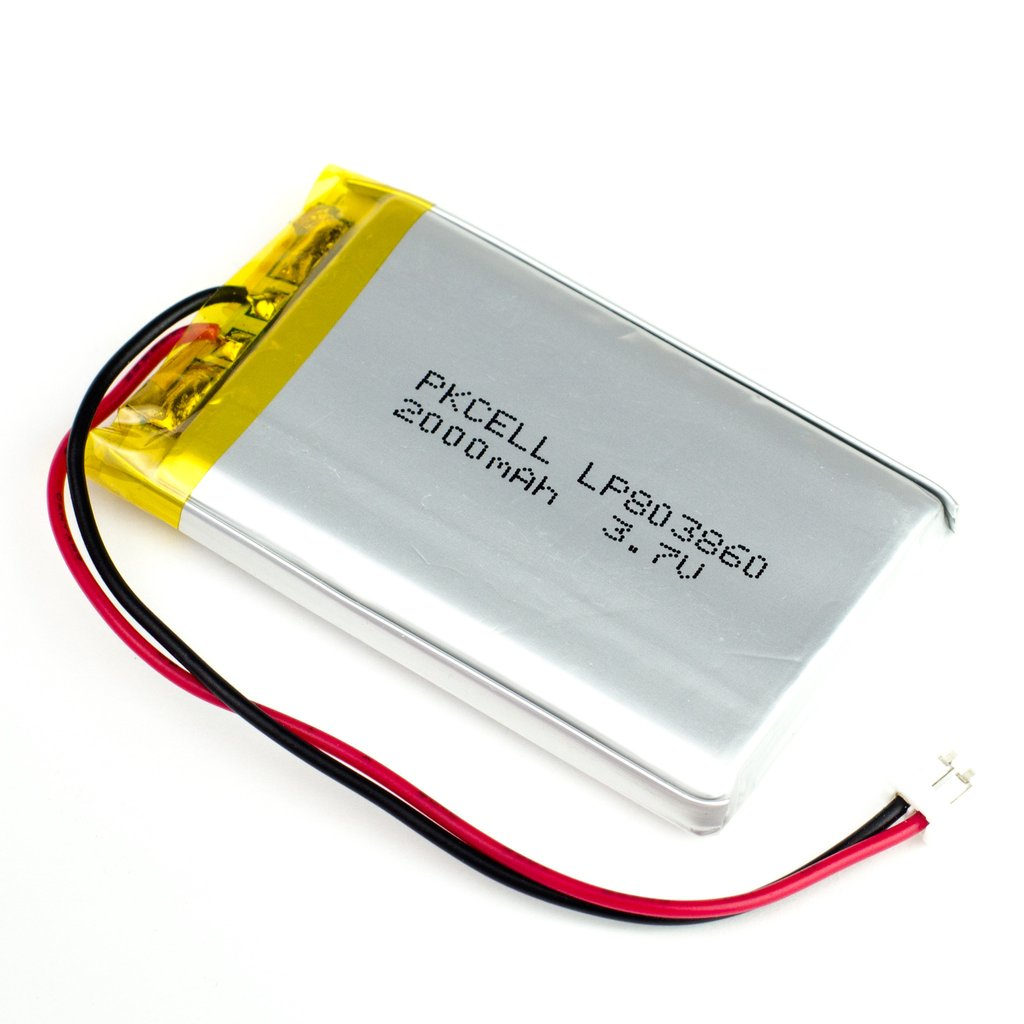
\includegraphics[width=.35\linewidth]{graphics/lipo}\\
    \vfill
    \scalebox{2}{$$3.0V\;\rightarrow\;4.2V \quad\Rightarrow\quad 3.3V$$}
    \vfill
\end{frame}

\begin{frame}{Software Design}
	\begin{figure}
	\centering
	  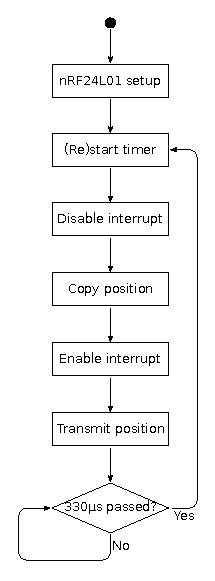
\includegraphics[width=.25\linewidth]{graphics/joint_software_diagram}
	\end{figure}
\end{frame}


%\begin{frame}{Software Design}
%	\begin{figure}
%	\centering
%	  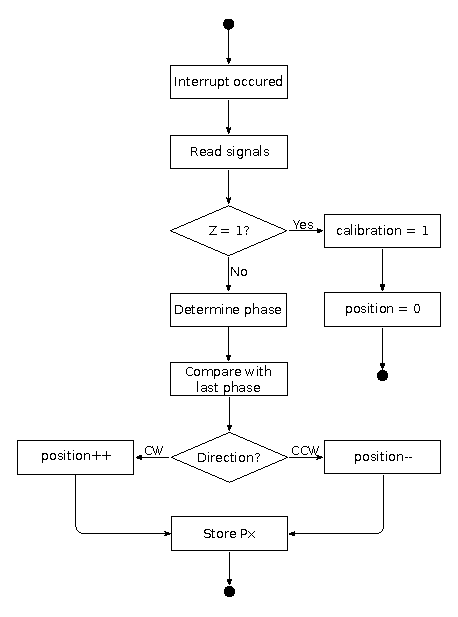
\includegraphics[width=.55\linewidth]{graphics/joint_interrupt}
%	\end{figure}
%\end{frame}

\begin{frame}[c]{Test Columns}
\begin{columns}
\column{.5\linewidth}
\textbf{Solutions:}   
\begin{itemize}
			\item Buck converter
			\item Buck-Boost converter
			\item Linear regulator
\end{itemize}
\column{.5\linewidth}
\textbf{Parameters:}
\begin{itemize}
			\item Efficiency
			\item Drop out voltage
			\item []
\end{itemize}
\end{columns}
\end{frame}

\begin{frame}[c]\frametitle{Buck Converter}
	\begin{equation}
		V_{drop} = I_{O} \cdot (R_{DS(on)}+R_I)
		\label{eq:drop_v_tps62}
	\end{equation}

	\begin{equation}
		V_{drop} = 0.02 \cdot (0.062+0.09) = 14 [mV]
		\label{eq:drop_v_tps62_2}
	\end{equation}

	\begin{equation}
		\eta \approx 95\%
	\end{equation}
\end{frame}

\begin{frame}[c]\frametitle{Comparison}
	\begin{table}[h]
		\begin{tabular}{l|c|c|c}
			  ~				& \textbf{Buck} 	& \textbf{Buck-Boost}& \textbf{Linear}\tabularnewline 
			 Efficiency  	& 95\% 	& 75\%		& 89\%	\\
			 Drop out [mV]	& 14  	& N/A		& 20	\\
		\end{tabular}
	\end{table}
\end{frame}

\begin{frame}[t]\frametitle{Battery Characteristics}
    \begin{figure}[h]
		\centering
		% This file was created by matlab2tikz.
%
%The latest updates can be retrieved from
%  http://www.mathworks.com/matlabcentral/fileexchange/22022-matlab2tikz-matlab2tikz
%where you can also make suggestions and rate matlab2tikz.
%
\definecolor{mycolor1}{rgb}{0.00000,0.44700,0.74100}%
%
\begin{tikzpicture}

\begin{axis}[%
width=4.521in,
height=3.566in,
at={(0.758in,0.481in)},
scale only axis,
xmin=0,
xmax=450,
xlabel style={font=\color{white!15!black}},
xlabel={Time [Min]},
ymin=2.5,
ymax=4.5,
ytick={2.5,   3, 3.5,   4, 4.5},
ylabel style={font=\color{white!15!black}},
ylabel={Voltage [V]},
axis background/.style={fill=white},
title style={font=\bfseries},
title={Discharge Curve of Li-Ion Battery}
]
\addplot [color=mycolor1, forget plot]
  table[row sep=crcr]{%
0	4.072\\
10	4.02699999999999\\
20	4.00799999999998\\
40	3.95999999999998\\
50	3.92200000000003\\
60	3.89499999999998\\
70	3.87900000000002\\
80	3.85500000000002\\
90	3.84300000000002\\
100	3.81799999999998\\
110	3.79700000000003\\
120	3.78899999999999\\
130	3.77699999999999\\
140	3.767\\
150	3.75299999999999\\
160	3.76100000000002\\
170	3.75999999999999\\
180	3.74000000000001\\
190	3.72500000000002\\
200	3.71300000000002\\
210	3.714\\
220	3.69999999999999\\
230	3.71100000000001\\
240	3.71199999999999\\
250	3.69999999999999\\
260	3.69299999999998\\
270	3.69099999999997\\
280	3.69799999999998\\
290	3.69099999999997\\
300	3.68099999999998\\
310	3.673\\
320	3.65699999999998\\
330	3.64499999999998\\
340	3.63499999999999\\
350	3.62299999999999\\
360	3.60700000000003\\
370	3.61399999999998\\
380	3.596\\
390	3.56799999999998\\
400	3.505\\
410	3.36099999999999\\
414.551694551695	2.30000000000001\\
};
\addplot [color=red, dashed, forget plot]
  table[row sep=crcr]{%
0	3.30000000000001\\
450	3.30000000000001\\
};
\end{axis}
\end{tikzpicture}%
	\end{figure}
\end{frame}

\begin{frame}[c]\frametitle{Designed PCB}
	\begin{figure}
	\centering
	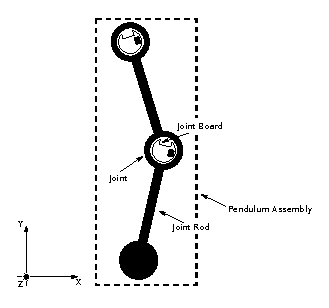
\includegraphics[width=.7\linewidth]{graphics/joint_assembly}
	\end{figure}
\end{frame}

\begin{frame}[standout]
  Questions?
\end{frame}

\end{document}